\documentclass[11pt]{article}
    \title{\textbf{Práctica 3}}
    \author{Daniel Linares Bernal}
    \date{24/12/2022}
    
    \addtolength{\topmargin}{-3cm}
    \addtolength{\textheight}{3cm}
\usepackage{graphicx}
\begin{document}

\maketitle
\thispagestyle{empty}

\section{TM solución de el ejercicio 3.4}
\begin{figure}[h]
\centering
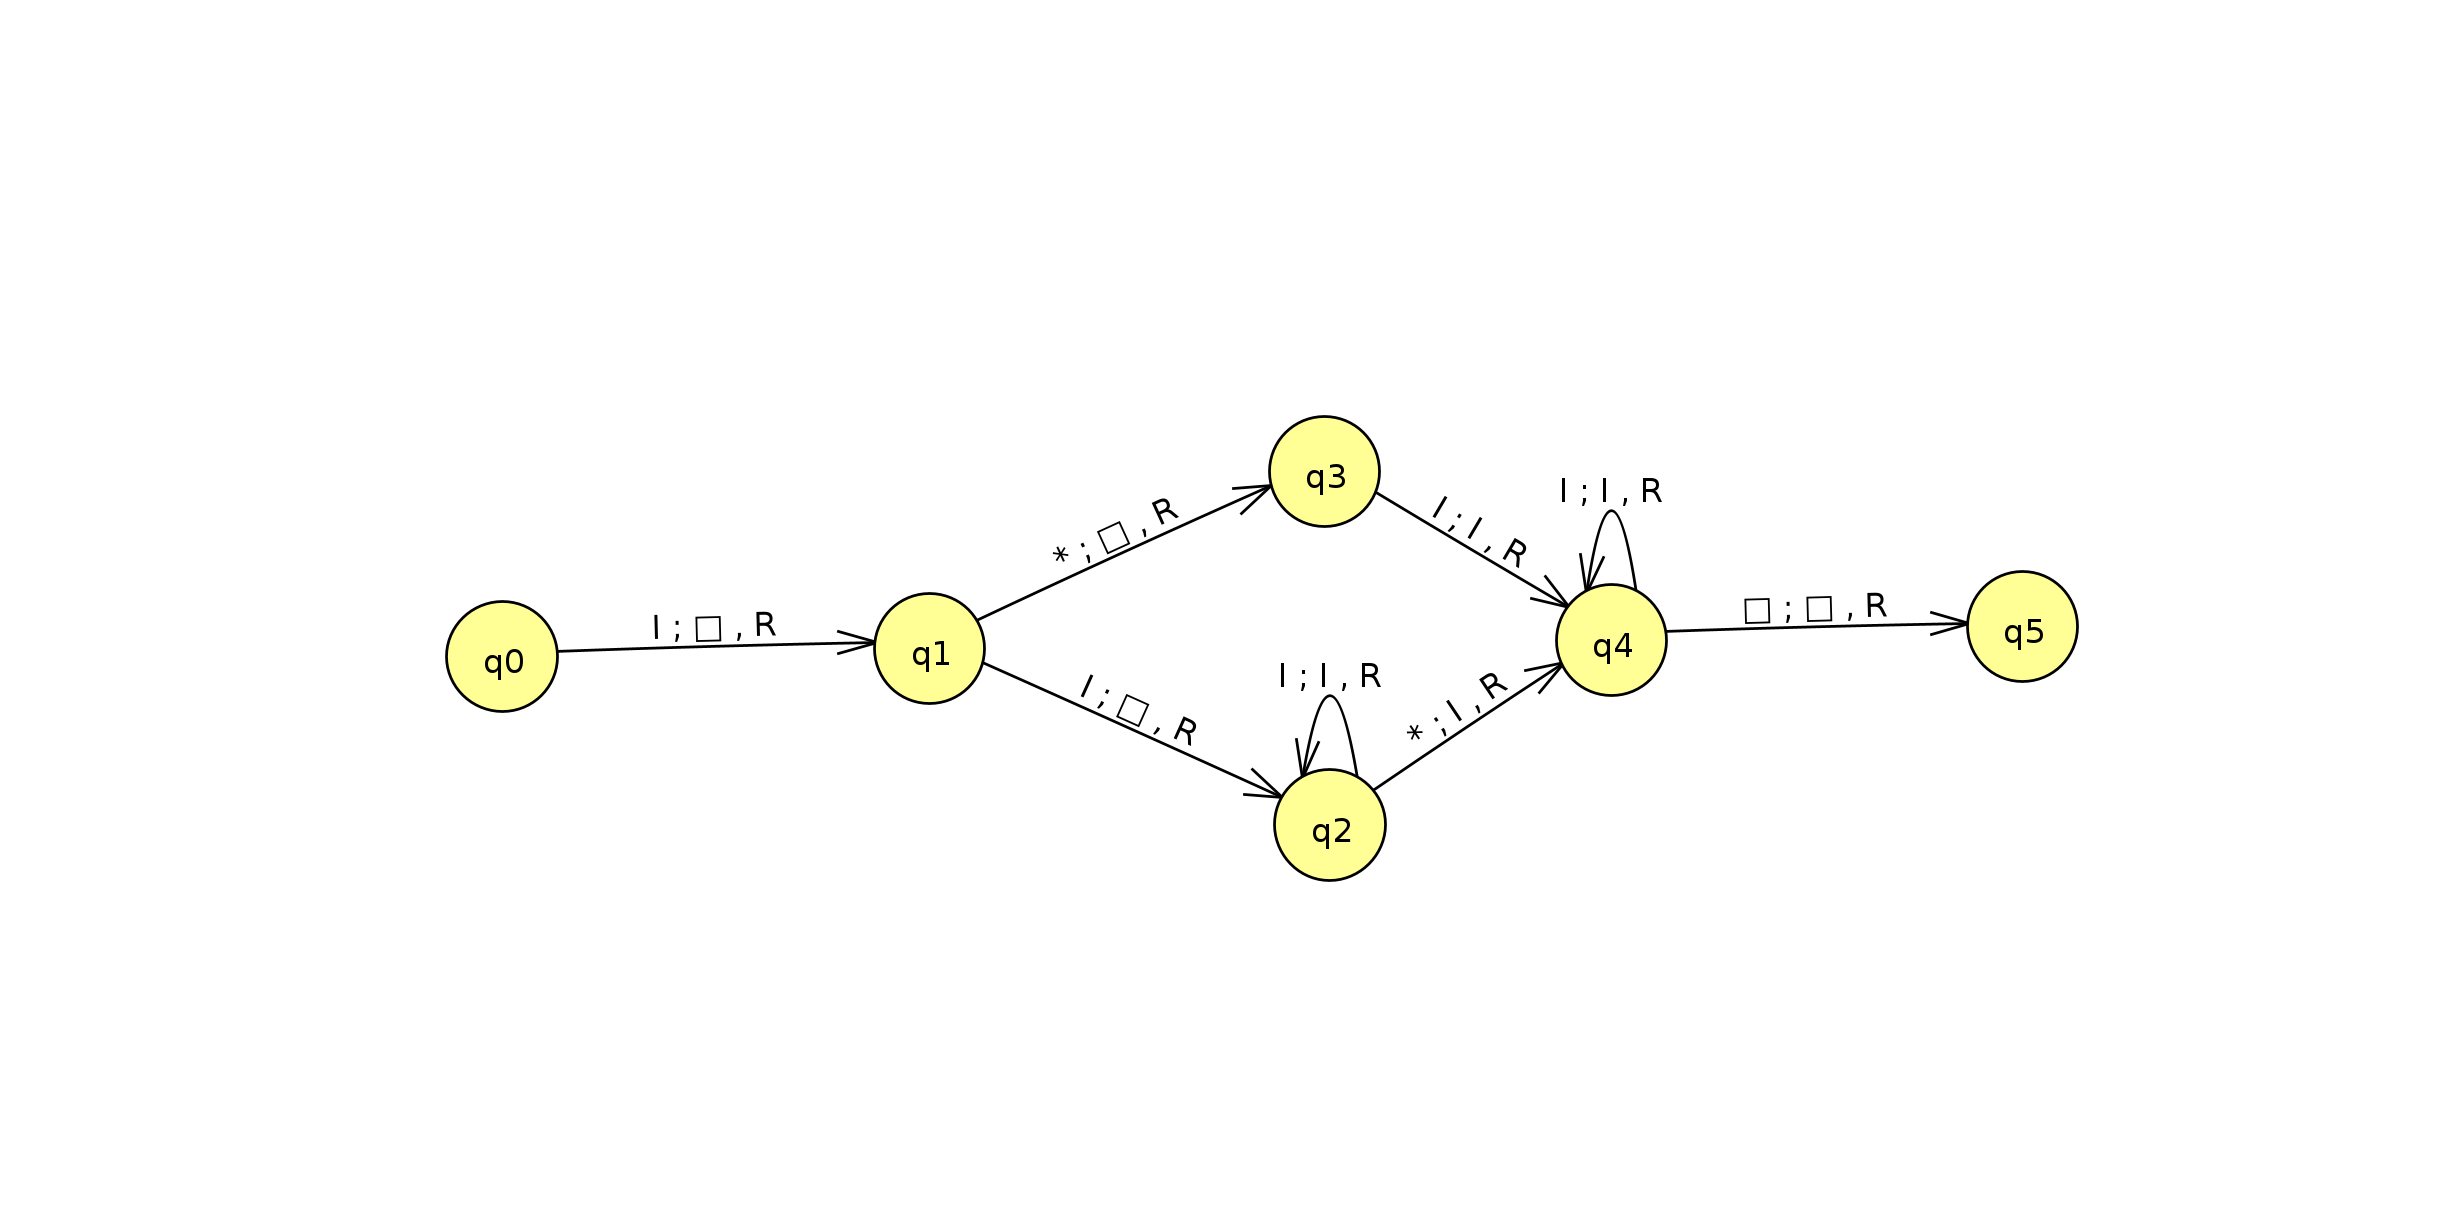
\includegraphics[width=1.2\linewidth]{TM.png}
\end{figure}

\section{Suma de tres valores de forma recursiva}
Suma3 : N³ $\rightarrow$ N\\ Suma3(x,y,z) = x + y + z\\\\
Suma3 = $\langle \pi_1^1$ $|$ $successor_4 \rangle$ where\\\\
$successor_4$ : N elevado a 4 $\rightarrow$ N\\
$successor_4(x,y,z,t) = t + 1$\\
$successor_4$ = $\sigma  (\pi_4^4)$\\\\
Suma3 = $\langle \pi_1^1$ $|$ $\sigma(\pi_4^4)$

\section{Suma de tres valores en lenguaje WHILE}

Usaremos X4 como auxiliar para almacenar el resultado de la suma (se puede usar X1 y queda más corto pero lo he entendido así), y haremos un bucle while por cada valor que queremos sumar, sumando 1 a X4 y restando 1 al valor tantas veces hasta que sea 0, quedando así:\\\\
X4 := 0\\
while X1 $\neq$ 0 do\\
	X4 := X4 + 1\\
	X1 := X1 - 1\\
od\\
while X2 $\neq$ 0 do\\
	X4 := X4 + 1\\
	X2 := X2 - 1\\
od\\
while X3 $\neq$ 0 do\\
	X4 := X4 + 1\\
	X3 := X3 - 1\\
od\\
\end{document}